\documentclass[../main.tex]{subfiles}

\begin{document}
    \begin{itemize}
        \item Zarządzanie strategicznie,
        \item Zarządzanie operacyjne,
        \item Zarządzanie zespołem testowym.
    \end{itemize}

    \subsection{Testowanie oparte na ryzyku.}

    \textbf{Ryzyko} – możliwość (prawdopodobieństwo) wystąpienia negatywnego lub niepożądanego zdarzenia.

    \textbf{Poziom ryzyka} – ważność ryzyka określona przez prawdopodobieństwo i wpływ; może być ilościowy lub
    jakościowy.

    \textbf{Zarządzanie ryzykiem} - w podejściu opartym na ryzyku ryzyko jest podstawową bazą testów.

    \begin{figure}[H]
        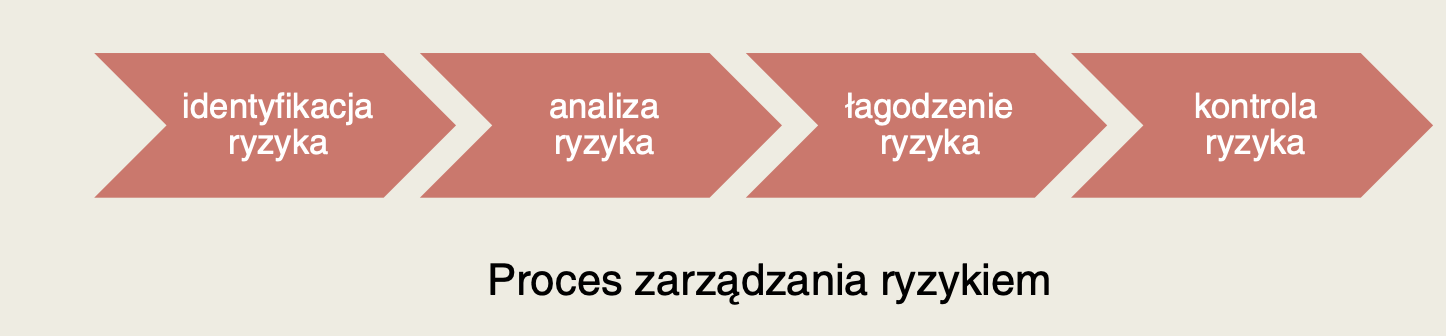
\includegraphics[width=\linewidth]{ryzyko.png}
    \end{figure}

    \begin{table}[H]
        \begin{center}
            \begin{tabular}{| p{8cm}  p{8cm} |}
                \hline
                \multicolumn{2}{|c|}{\textbf{Identyfikacja ryzyka}}\\
                \multicolumn{2}{|c|}{proces identyfikacji możliwych do wystąpienia ryzyk. Techniki identyfikacji
                ryzyka:}\\
                \hline
                \begin{itemize}
                    \item burza mózgów
                    \item listy kontrolne
                    \item historia awarii
                    \item wywiady eksperckie
                \end{itemize}
                &
                \begin{itemize}
                    \item szablony ryzyk
                    \item niezależna ocena
                    \item doświadczenie z poprzednich projektów
                \end{itemize}\\
                \hline
                \hline
                \multicolumn{2}{|c|}{\textbf{Łagodzenie ryzyka}}\\
                \multicolumn{2}{|c|}{proces implementacji planów mających zapobiegać ryzyku. Metody łagodzenia ryzyka:}\\
                \hline
                \begin{itemize}
                    \item łagodzenie ryzyka przez podjęcie \textbf{czynności prewencyjnych}, zapobiegających pojawieniu się ryzyka lub zmiejszających ich ewentualną dotkliwość
                    \item \textbf{plany awaryjne} mające na celu redukcję siły oddziaływania ryzyka, które wystąpi
                \end{itemize}
                &
                \begin{itemize}
                    \item \textbf{transfer ryzyka}, czyli przeniesienie ryzyka na stronę trzecią (np. ubezpieczyciela), który ponosi skutki wystąpienia ryzyka
                    \item \textbf{zignorowanie i zaakceptowanie ryzyka}, czyli niepodejmowanie żadnych akcji do mommentu wystąpienia ryzyka
                \end{itemize}\\
                \multicolumn{2}{|p{16cm}|}{Podczas fazy łagodzenia ryzyka następuje priorytetyzacja testów wg poziomu ryzyka. Poziom ryzyka wpływa na zakres testowania.}\\
                \hline
                \hline
                \multicolumn{2}{|c|}{\textbf{Kontrola (monitorowanie) ryzyka}}\\
                \multicolumn{2}{|c|}{ciągła obserwacja aktualnego stanu systemu Przykładowe metryki zbierane w ramach procesu:}\\
                \hline
                \begin{itemize}
                    \item \% pokrytych wymagań
                    \item \% pokrytych funkcjonalności
                    \item \% testów zdanych/nie zdanych
                    \item poziom zminimalizowanego i rezydualnego ryzyka
                \end{itemize}
                &
                \begin{itemize}
                    \item ryzyka w podziale na:
                    \begin{itemize}
                        \item zminimalizowane (odpowiadające testy przeszły)
                        \item "w trakcie" (wykryto problemy)
                        \item niepokryte (nie uruchomiono jeszcze odpowiadających testów)
                    \end{itemize}
                \end{itemize}\\
                \hline
            \end{tabular}
        \end{center}
    \end{table}

    \subsubsection{Analiza ryzyka}
    Proces \textbf{oceny zidentyfikowanych ryzyk} w celu \textbf{oszacowania} ich \textbf{wpływu}
    oraz \textbf{prawdopodobieństwa} wystąpienia. Wyjście: lista ryzyk z przypisanymi poziomami/priorytetami ryzyk, określeniem zakresu testowania, metod zapobiegania ryzykom na podstawie oceny czynników technicznych i biznesowych poziomu ryzyka.

    \textbf{Szacowanie ilościowe} analizy ryzyka to określenie kosztu materializacji ryzyka.
    Często trudne lub niemożliwe – wtedy stosuje się \textbf{podejście jakościowe}.

    \begin{table}[H]
        \begin{center}
            \begin{tabular}{| p{8cm} | p{8cm} |}
                \hline
                \multicolumn{2}{|c|}{\textbf{Metody analizy ryzyka}}\\
                \hline
                \hline
                \textbf{FMEA (Failure Mode and Effect Analysis)} & \textbf{FTA (Fault Tree Analysis)}\\
                \begin{itemize}
                    \item Podejście do \textbf{systematycznej identyfikacji możliwych awarii} systemu
                    \item Awarie są priorytetyzowane wg:
                    \begin{itemize}
                        \item konsekwencji ich wystąpień
                        \item prawdopodobieństwa(częstości)wystąpień – łatwości ich wykrycia
                    \end{itemize}
                    \item Cel FMEA: podjęcie akcji w celu \textbf{eliminacji lub redukcji awarii}, poczynając od najpoważniejszych
                \end{itemize}
                &
                \begin{itemize}
                    \item Inaczej analiza drzewa usterek
                    \item Metoda analizy niezawodności, bezpieczeństwa i utrzymywalności
                    \item Dedukcyjna procedura używana w celu określenia \textbf{różnych kombinacji awarii} software’u, hardware’u i błędów ludzkich, które mogą wywołać niepożądane efekty na poziomie systemowym
                    \item Podejście \textbf{top-down} (od ogółu – awarii systemowej, do szczegółu – pojedynczych błędów na niskich poziomach). Podstawowe elementy to bramki logiczne.
                \end{itemize}\\
                \hline
                \textbf{QFD (Quality Function Deployment)}
                &
                \textbf{PRisMa (Product Risk Management)}\\
                &
                \begin{itemize}
                    \item prawdopodobieństwo i wpływ traktowane osobno, nie łącznie
                \end{itemize}
                \\
                \hline
            \end{tabular}
        \end{center}
    \end{table}

    \begin{figure}[H]
        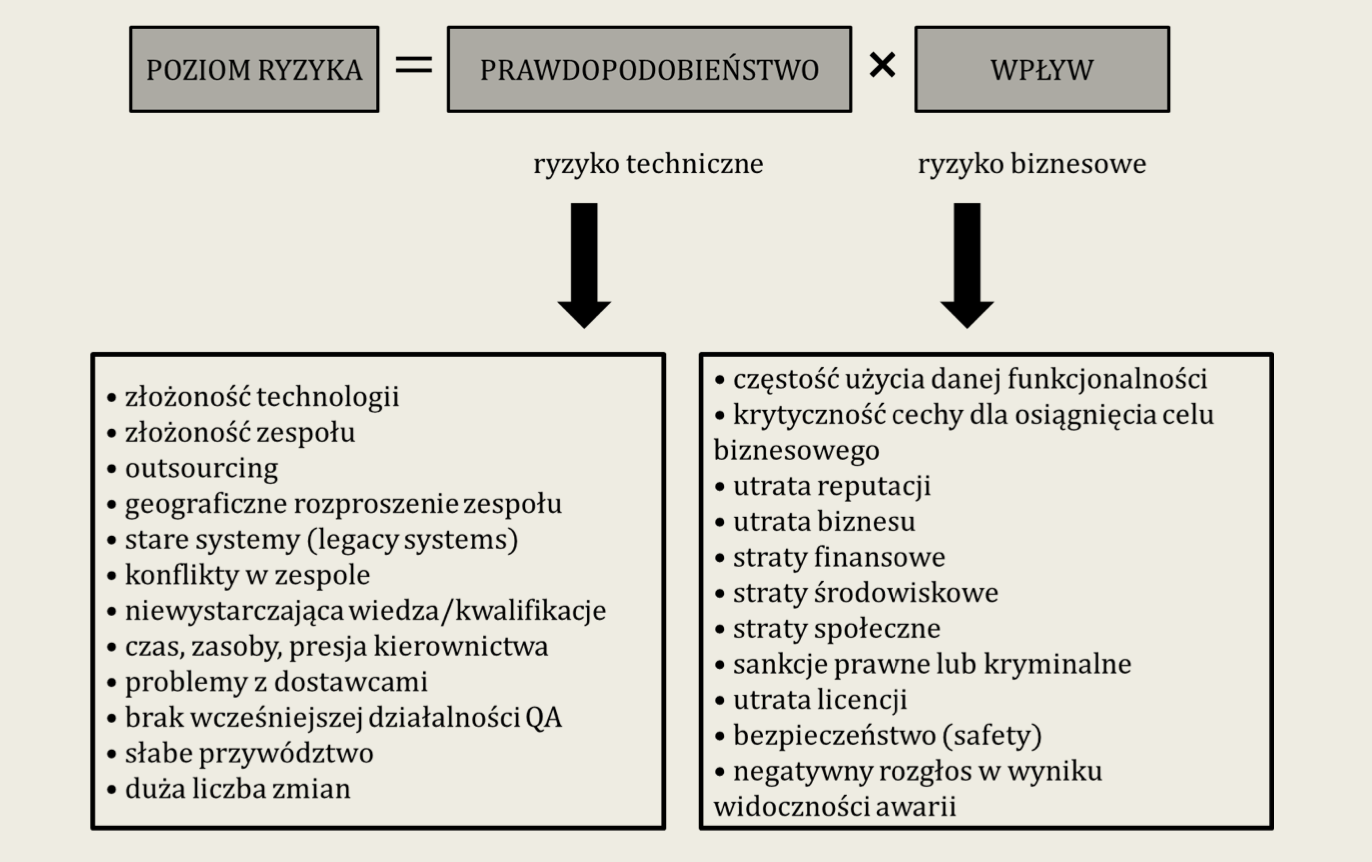
\includegraphics[width=\linewidth]{analiza_ryzyka.png}
    \end{figure}



    \subsection{Biznesowa wartość testowania.}

    \textbf{Model CoQ} (Cost of (Poor) Quality) - model opisujący \textbf{koszty} związane z dostarczeniem
    produktu lub usługi o \textbf{niskiej jakości}.
    Rodzaje kosztów

    \begin{table}[H]
        \begin{center}
            \begin{tabular}{| p{5cm} || p{11cm} |}
                \hline
                \textbf{Rodzaj kosztów} & \textbf{Powód ich ponoszenia}\\
                \hline
                \hline
                koszty \textbf{zapobiegania} & aby unikać defektów; dot. wymagań, planowania i zapewniania jakości, szkoleń (np. szkolenie deweloperów, aby pisany kod był lepszej jakości)\\
                \hline
                koszty \textbf{wykrywania} & aby wykrywać defekty; ponoszone nawet, gdy nie wykryjemy żadnych defektów (np. wydatki na analizę, projektowanie, implementację, niektóre koszty wykonania testów)\\
                \hline
                koszty \textbf{wewnętrznego błędu} & z powodu wykrycia awarii (np. pozostałe koszty wykonania testów, koszty re-testów, koszt naprawy defektu przez programistę)\\
                \hline
                koszty \textbf{zewnętrznego błędu} & z powodu niewykrycia awarii (np. koszty wsparcia technicznego, helpdesku, naprawy defektów polowych, kary umowne)\\
                \hline
            \end{tabular}
        \end{center}
    \end{table}

\end{document}